%
% Modified by Megan Patnott
% Last Change: Jan 18, 2013
%
%%%%%%%%%%%%%%%%%%%%%%%%%%%%%%%%%%%%%%%%%%%%%%%%%%%%%%%%%%%%%%%%%%%%%%%%
%
% Modified by Bryce Frentz
% Last Change: 2018
%
%%%%%%%%%%%%%%%%%%%%%%%%%%%%%%%%%%%%%%%%%%%%%%%%%%%%%%%%%%%%%%%%%%%%%%%%
%
% Sample Notre Dame Thesis/Dissertation
% Using Donald Peterson's ndthesis classfile
%
% Written by Jeff Squyres and Don Peterson
%
% Provided by the Information Technology Committee of
%   the Graduate Student Union
%   http://www.gsu.nd.edu/
%
% Nothing in this document is serious except the format.  :-)
%
% If you have any suggestions, comments, questions, please send e-mail
% to: ndthesis@gsu.nd.edu
%
%%%%%%%%%%%%%%%%%%%%%%%%%%%%%%%%%%%%%%%%%%%%%%%%%%%%%%%%%%%%%%%%%%%%%%%%

%
% Chapter 3
%

\chapter{Cross section data Reduction and analysis}
\label{chap: data}

\section{Introduction}

In aggregate, the data taken at both the CASPAR and NSL experiments consists of $\gamma$-ray energy data from the $^{14}$N$\left( p,\gamma \right) ^{15}$O reaction, observed with a single, 130\% HPGe detector placed at $55^{\degree}$ relative to the beam direction. These data were collected for reactions over the combined proton energy range of 270 - 1200 keV. The primary interest of these experiments was monitoring the R/DC$\rightarrow$GS transition and the R/DC$\rightarrow$6.79 MeV + 6.79 MeV$\rightarrow$GS transition sequence. As such, the energies of the concerned photons ranged in energy from $\sim$600 keV up to $\sim$8500 keV. This chapter details the processes by which this data is gathered and turned into an experimental cross section.

\section{Angular corrections}
\label{sec: angularCorrections}

The angular distribution of a cross section, $W$, can be described by

\begin{equation}
W_{\text{exp}} = a_{0} \left(1 + \sum_{i = 1}^{n} a_{i} Q_{i} P_{i} ( \cos (\theta) )    \right)
\end{equation}

\noindent where $a_{i}$ are the angular distribution coefficients, $Q_{i}$ are correction factors due to the finite size of a given detector, and the $P_{i} ( \cos (\theta) )$ are the Legendre polynomials of order $i$. For the conditions of this work, odd numbered terms as well as those of order higher than 2 give negligible contribution to the angular distribution. Therefore, the resulting angular distribution of this reaction is of the form

\begin{equation}
W_{\text{exp}} = a_{0} + a_{2} Q_{2} P_{2} ( \cos (\theta) ).
\end{equation}

Experimentally, to address any effects arising from an angular distribution of this form, the detector was placed at $55^{\degree}$. This is the zero of the 2nd order Legendre polynomial, thereby minimizing any effects on the cross section arising from the detector's angle. Simultaneously, this means that no correction of the data is necessary.


\section{Energy calibration}
\label{sec: energy calibration}

It is important to establish the true relationship between $\gamma$-rays of different energies incident in a detector and the signal they produce during data acquisition. This connection is determined by calibrating the system with $\gamma$-rays of well-known energy from room background, given radioactive sources, like $^{137}$Cs or $^{60}$Co, and well-studied nuclear reactions, like $^{27}$Al($p, \gamma$)$^{28}$Si. The reactions are also used in calibration because no natural sources of radioactivity provide $\gamma$'s with energy higher than 3.6 MeV, whereas the $^{27}$Al($p, \gamma$)$^{28}$Si reaction provides $\gamma$ ray energies up to 10.7 MeV, ensuring that the detector is well calibrated over the entire energy range for $\gamma$'s that will be seen in the $^{14}$N$\left( p,\gamma \right) ^{15}$O reaction. The exact relationship between the the channel number in the acquisition system analog-to-digital converter (ADC) and the incident photon energy, $E_{\gamma}$, is characterized by the standard linear relationship

\begin{equation}
E_{\gamma} = m \times \text{Channel} + b
\end{equation}

\noindent where $m$ is simply the slope and $b$ the offset of the fit. For a HPGe detector, a linear relationship is sufficient and appropriate to describe the ADC response. However, this process was redone for every phase of the experiment because slightly different gains applied to the ADC's and signal amplifiers provide a different relationship in the electronics. Therefore, despite using the same detector, each phase of the experiment required its own energy calibration, an example of which is shown in Fig.\ \


\begin{figure}
\centering
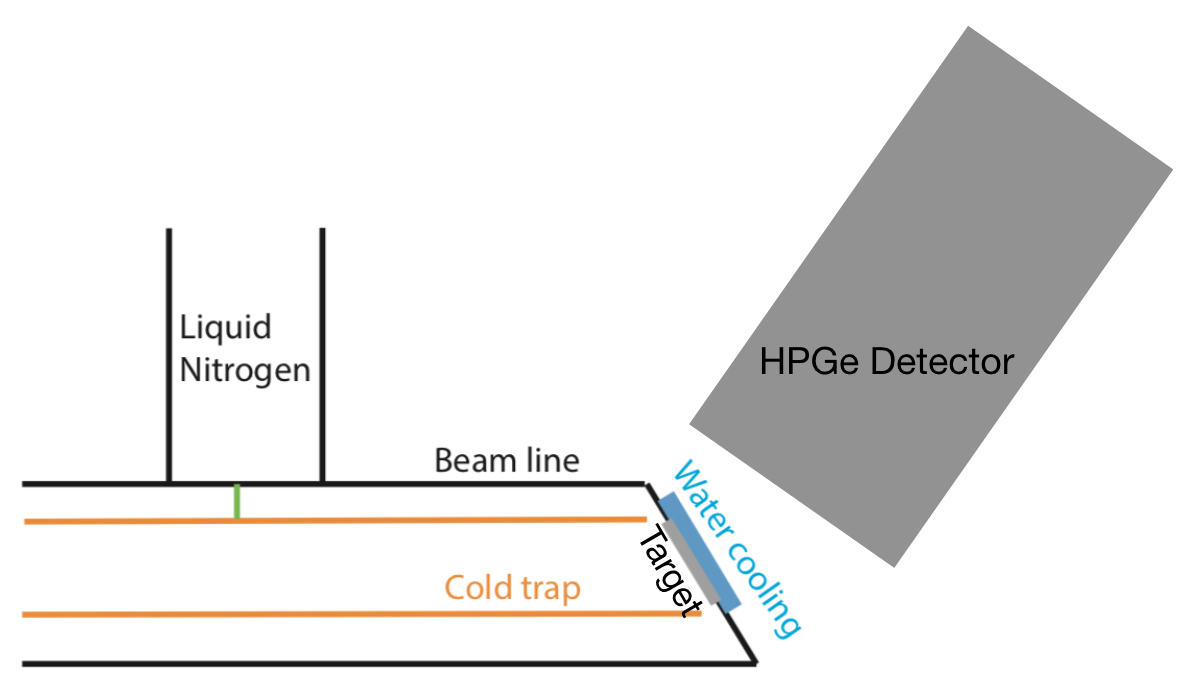
\includegraphics[width=0.8\linewidth]{figures/expSetup.png}
\label{fig: energyCalibration}
\caption{Energy calibration curve for the HPGe detector taken at CASPAR. The calibration incorporated natural background, radioactive sources, and the products from the $^{27}$Al($p, \gamma$)$^{28}$Si reaction. }
\end{figure}




\section{Efficiency}
\label{sec: efficiency}



\subsection{Total efficiency}

\subsection{Full energy peak efficiency}


\section{Summing corrections}
\label{sec: summing}

\section{Target characterization}
\label{sec: target}

\section{Cross-section determination}
\label{sec: cross-section}





% % uncomment the following lines,
% if using chapter-wise bibliography
%
% \bibliographystyle{ndnatbib}
% \bibliography{example}
